\section{Invariant Attacks -- Round Constants}
\begin{frame}[plain]
    \sectionpage
    \vfill
\end{frame}

\begin{frame}{Invariant Attacks}
    \begin{block}{Main Idea: Invariant Subspaces}
        \centering
        \vspace{0.25em}
        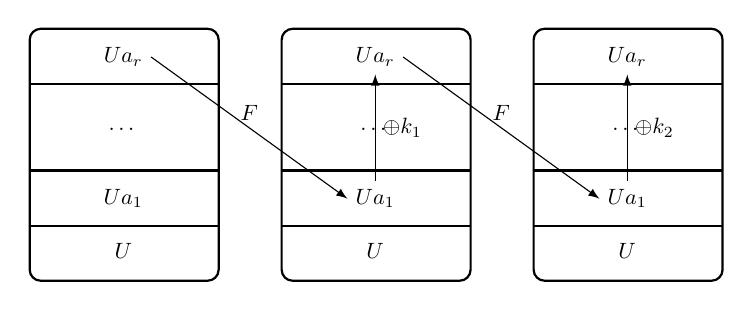
\begin{tikzpicture}[scale=0.8]
            \tikzstyle{every node}=[transform shape];

            \node (left-space) [draw,rectangle,thick,rounded corners,minimum width=3cm,minimum height=4cm,fill=white] at (1,0) {};
            \draw[thick] (left-space.west)+(0,1.125cm) -- node[above, yshift=1.5mm] (uar1) {$\coset{U}{a_r}$} +(3cm,1.125cm);
            \draw[thick] (left-space.west)+(0,-0.25cm) -- node[above, yshift=5mm] {\dots} +(3cm,-0.25cm);
            \draw[thick] (left-space.west)+(0,-1.125cm) -- node[above, yshift=1.5mm] {$\coset{U}{a_1}$}
                                                           node[below, yshift=-1.5mm] {$U$} +(3cm,-1.125cm);

            \node (middle-space) [draw,rectangle,thick,rounded corners,minimum width=3cm,minimum height=4cm,fill=white] at (5,0) {};
            \draw[thick] (middle-space.west)+(0,1.125cm) -- node[above, yshift=1.5mm] (uar2) {$\coset{U}{a_r}$} +(3cm,1.125cm);
            \draw[thick] (middle-space.west)+(0,-0.25cm) -- node[above, yshift=5mm] {\dots} +(3cm,-0.25cm);
            \draw[thick] (middle-space.west)+(0,-1.125cm) -- node[above, yshift=1.5mm] (ua12) {$\coset{U}{a_1}$}
                                                           node[below, yshift=-1.5mm] {$U$} +(3cm,-1.125cm);

            \draw[-latex] (uar1.east) -- node[above] {$F$} (ua12.west);
            \draw[-latex] (ua12.north) -- node[right] {$\oplus k_1$} (uar2.south);

            \visible<2->{%
            \node (right-space) [draw,rectangle,thick,rounded corners,minimum width=3cm,minimum height=4cm,fill=white] at (9,0) {};
            \draw[thick] (right-space.west)+(0,1.125cm) -- node[above, yshift=1.5mm] (uar3) {$\coset{U}{a_r}$} +(3cm,1.125cm);
            \draw[thick] (right-space.west)+(0,-0.25cm) -- node[above, yshift=5mm] {\dots} +(3cm,-0.25cm);
            \draw[thick] (right-space.west)+(0,-1.125cm) -- node[above, yshift=1.5mm] (ua13) {$\coset{U}{a_1}$}
                                                           node[below, yshift=-1.5mm] {$U$} +(3cm,-1.125cm);

            \draw[-latex] (uar2.east) -- node[above] {$F$} (ua13.west);
            \draw[-latex] (ua13.north) -- node[right] {$\oplus k_2$} (uar3.south);
            }
        \end{tikzpicture}
    \end{block}
    \visible<3->{%
    \begin{block}{Invariant Subspace Attacks~[Lea+11] (CRYPTO'11)}
        \vspace{0.25em}
        Let $U \subseteq \F_2^n$, $c, d \in U^\perp$, and $F : \F_2^n \to \F_2^n$.
        Then $U$ is an \emph{invariant subspace} (IS) if and only if
            $F(\coset{U}{c}) = \coset{U}{d}$
        and all round keys in $\coset{U}{(c+d)}$ are \emph{weak keys}.
    \end{block}
    }
\end{frame}

\begin{frame}{Invariant Attacks}{A Short History}
    \begin{timeline}
        \Task[\cite{C:LAAZ11}]{Publication of IS attack, breaking \printcipher/}
        \Task[\cite{EC:LeaMinRon15}]{Generic Algorithm to find ISes, breaking \robin/, \iscream/, \zorro/}
        \Task[\cite{ToSC:GJNQSM16}]{IS attack breaking \midori/64}
        \Task[\cite{AC:TodLeaSas16}]{Invariant Set generalisation, breaking \scream/, \iscream/, \midori/64}
        \Task[\cite{C:BCLR17}]{Proving resistance for Invariant attacks}
    \end{timeline}
\end{frame}

\begin{frame}{Invariant Attacks}{Proving Resistance}
    \centering
    \begin{block}{\textbf{Goal}: Apply security argument from}
    \begin{quote}
        \fullcite{C:BCLR17}.
    \end{quote}
    \end{block}
    \begin{exampleblock}{What do we get from this?}
        \begin{itemize}
            \item Non-existence of invariants for both parts of the ronud function (S-box and linear layer)
        \end{itemize}
    \end{exampleblock}
    \begin{alertblock}{Issues}
    \begin{itemize}
        \item Other partitionings of the round function might allow invariants (Christof B\@. found examples)
        \item Not clear how to prove the general absence of invariant attacks (best we can currently prove)
        \item All known attacks exploit exactly this structure (splitting in S-box and linear layer)
    \end{itemize}
    \end{alertblock}
\end{frame}

\begin{frame}{Invariant Attacks}{Recap Security Argument (I)}
    \begin{columns}
        \begin{column}{0.35\textwidth}
        \begin{block}{Observation}
            \begin{itemize}
                \item Invariants for the linear layer $L$ and round key addition have to contain special linear structures.
                \item Denote by $c_1, \dots, c_t$ the round constant differences for rounds with the same round key.
                \item Then the linear structures of any invariant have to contain $W_L(c_1, \dots, c_t)$.
            \end{itemize}
        \end{block}
        \pause
    \end{column}
    \begin{column}{0.6\textwidth}
    \begin{block}{Linear Structures}
        Let $f : \F_2^n \to \F_2$.
        Then its \emph{linear structures} are
        \vspace*{-5pt}
        \begin{equation*}
            \mathrm{LS} \coloneqq \set{a \given f(x) + f(x+a) \text{ is constant}}\;.
        \end{equation*}
        \vspace*{-15pt}
    \end{block}
    \begin{block}{The smallest $L$-invariant subspace}
        $W_L(c_1, \dots, c_t)$ is the \emph{smallest $L$-invariant subspace} of~$\F_2^n$ containing all~$c_i$
        \vspace*{-5pt}
        \begin{equation*}
            \Leftrightarrow \forall x \in W_L(c_1, \dots, c_t): L(x) \in W_L(c_1, \dots, c_t)
        \end{equation*}
        \vspace*{-15pt}
    \end{block}
    \pause
    \begin{exampleblock}{The simple case}
        If $W_L(c_1, \dots, c_t) = \F_2^n$, only trivial invariants for $L$ and key addition are possible (constant 0 and 1 function).
    \end{exampleblock}
    \end{column}
    \end{columns}
\end{frame}

\begin{frame}{Invariant Attacks}{Recap Security Argument (II)}
    \begin{block}{Application to \clyde/}
    \begin{columns}
        \begin{column}{0.55\textwidth}
        \begin{itemize}
            \item Find the important round constant differences:\\
                  {\small (the differences where the same tweakey is added)}
        \end{itemize}
        \end{column}
        \pause
            \begin{column}{0.45\textwidth}
            \begin{itemize}
                \item[] Set of RC differences $D$ below\\
                        with $\abs{D} = 20$
            \end{itemize}
            \end{column}
    \end{columns}
    \end{block}
    \begin{columns}
        \visible<3->{
        \begin{column}{0.49\textwidth}
            \begin{tikzpicture}[background rectangle/.style={fill=white}, show background rectangle]
                \begin{scope}[scale=0.75, transform shape]
                \tikzstyle{every node}=[transform shape];
                \tikzstyle{every node}=[node distance=25pt];

                \node (XOR11) [XOR,scale=1.2] {};

                \node [left of=XOR11] (x) {$x$};
                \path[line] (x) edge (XOR11);

                \foreach \i in {1, 2, 3, 4} {
                    \node (f1\i) [right of=XOR1\i,draw,rectangle,thick,rounded corners,minimum width=0.25cm,minimum height=0.75cm] {$R$};
                    \path[line] (XOR1\i) edge (f1\i);
                    \pgfmathtruncatemacro\tmp{\i+1}
                    \node (XOR1\tmp) [right of=f1\i,XOR,scale=1.2] {};
                    \path[line] (f1\i) edge (XOR1\tmp);
                }

                \node (f21) [below=50pt of XOR15,draw,rectangle,thick,rounded corners,minimum width=0.25cm,minimum height=0.75cm] {$R$};
                \path[line] (XOR15.east) -- +(20pt,0) |- (f21.east);
                \node (XOR21) [left of=f21,XOR,scale=1.2] {};
                \path[line] (f21) edge (XOR21);

                \foreach \i in {2, 3, 4} {
                    \pgfmathtruncatemacro\tmp{\i-1}
                    \node (f2\i) [left of=XOR2\tmp,draw,rectangle,thick,rounded corners,minimum width=0.25cm,minimum height=0.75cm] {$R$};
                    \path[line] (XOR2\tmp) edge (f2\i);
                    \node (XOR2\i) [left of=f2\i,XOR,scale=1.2] {};
                    \path[line] (f2\i) edge (XOR2\i);
                }

                \node (f31) [below=50pt of XOR24,draw,rectangle,thick,rounded corners,minimum width=0.25cm,minimum height=0.75cm] {$R$};
                \path[line] (XOR24.west) -- +(-20pt,0) |- (f31.west);
                \node (XOR31) [right of=f31,XOR,scale=1.2] {};
                \path[line] (f31) edge (XOR31);

                \foreach \i in {2, 3, 4} {
                    \pgfmathtruncatemacro\tmp{\i-1}
                    \node (f3\i) [right of=XOR3\tmp,draw,rectangle,thick,rounded corners,minimum width=0.25cm,minimum height=0.75cm] {$R$};
                    \path[line] (XOR3\tmp) edge (f3\i);
                    \node (XOR3\i) [right of=f3\i,XOR,scale=1.2] {};
                    \path[line] (f3\i) edge (XOR3\i);
                }

                \node [right = 20pt of XOR34.east] (y) {$y$};
                \path[line] (XOR34) edge (y);

                \node (k00) [above=25pt of XOR11,marked on=<4>] {\small $\mathrm{TK}(0)$};
                \path[line,marked on=<4>] (k00) edge (XOR11);

                \node (k10) [above=25pt of XOR13,marked on=<5>] {\small $\mathrm{TK}(1)$};
                \path[line,marked on=<5>] (k10) edge (XOR13);

                \node (k20) [above=25pt of XOR15,marked on=<6>] {\small $\mathrm{TK}(2)$};
                \path[line,marked on=<6>] (k20) edge (XOR15);


                \node (k01) [above=25pt of XOR22,marked on=<4>] {\small $\mathrm{TK}(0)$};
                \path[line,marked on=<4>] (k01) edge (XOR22);

                \node (k11) [above=25pt of XOR24,marked on=<5>] {\small $\mathrm{TK}(1)$};
                \path[line,marked on=<5>] (k11) edge (XOR24);


                \node (k22) [above=25pt of XOR32,marked on=<6>] {\small $\mathrm{TK}(2)$};
                \path[line,marked on=<6>] (k22) edge (XOR32);

                \node (k02) [above=25pt of XOR34,marked on=<4>] {\small $\mathrm{TK}(0)$};
                \path[line,marked on=<4>] (k02) edge (XOR34);


                \node (w00) [below=25pt of XOR12,marked on=<7>] {\small $W(0)$};
                \path[line,marked on=<7>] (w00) edge (XOR12);

                \node (w10) [below=25pt of XOR13,marked on=<5>] {\small $W(1)$};
                \path[line,marked on=<5>] (w10) edge (XOR13);

                \node (w20) [below=25pt of XOR14,marked on=<7>] {\small $W(2)$};
                \path[line,marked on=<7>] (w20) edge (XOR14);

                \node (w30) [below=25pt of XOR15,marked on=<6>] {\small $W(3)$};
                \path[line,marked on=<6>] (w30) edge (XOR15);


                \node (w01) [below=25pt of XOR21,marked on=<7>] {\small $W(4)$};
                \path[line,marked on=<7>] (w01) edge (XOR21);

                \node (w11) [below=25pt of XOR22,marked on=<4>] {\small $W(5)$};
                \path[line,marked on=<4>] (w11) edge (XOR22);

                \node (w21) [below=25pt of XOR23,marked on=<7>] {\small $W(6)$};
                \path[line,marked on=<7>] (w21) edge (XOR23);

                \node (w31) [below=25pt of XOR24,marked on=<5>] {\small $W(7)$};
                \path[line,marked on=<5>] (w31) edge (XOR24);


                \node (w02) [below=25pt of XOR31,marked on=<7>] {\small $W(8)$};
                \path[line,marked on=<7>] (w02) edge (XOR31);

                \node (w12) [below=25pt of XOR32,marked on=<6>] {\small $W(9)$};
                \path[line,marked on=<6>] (w12) edge (XOR32);

                \node (w22) [below=25pt of XOR33,marked on=<7>] {\small $W(10)$};
                \path[line,marked on=<7>] (w22) edge (XOR33);

                \node (w32) [below=25pt of XOR34,marked on=<4>] {\small $W(11)$};
                \path[line,marked on=<4>] (w32) edge (XOR34);
            \end{scope}
            \end{tikzpicture}
        \end{column}
        \begin{column}{0.45\textwidth}
            \vspace*{-10pt}
            \begin{align*}
                             D &= {\only<4>{\color{alertred}}D_{\mathrm{TK}(0)}} \cup {\only<5>{\color{alertred}}D_{\mathrm{TK}(1)}} \cup {\only<6>{\color{alertred}}D_{\mathrm{TK}(2)}} \cup {\only<7>{\color{alertred}}D_0}\\[5pt]
                \visible<4->{\only<4>{\color{alertred}}D_{\mathrm{TK}(0)} &\only<4>{\color{alertred}}= \set{0 + W(5), 0 + W(11), W(5) + W(11)}} \\
                \visible<5->{\only<5>{\color{alertred}}D_{\mathrm{TK}(1)} &\only<5>{\color{alertred}}= \set{W(1) + W(7)}} \\
                \visible<6->{\only<6>{\color{alertred}}D_{\mathrm{TK}(2)} &\only<6>{\color{alertred}}= \set{W(3) + W(9)}} \\
                \visible<7->{\only<7>{\color{alertred}}D_{0} &\only<7>{\color{alertred}}= \set{a + b \given a, b \in D^\prime, a \neq b}} \\
                \visible<7->{\only<7>{\color{alertred}}D^\prime &\only<7>{\color{alertred}}= \set{W(0), W(2), W(4), W(6), W(8), W(10)}}
            \end{align*}
        \end{column}
        }
    \end{columns}
\end{frame}

\begin{frame}{Invariant Attacks}{Application to \clyde/}
    \begin{itemize}
        \item Computing $W_L$ is efficiently doable (takes $\approx$ 10 seconds on my laptop).
        \item For the round constants chosen for \clyde/, $\dim W_L(D) = 128 = n$.
    \end{itemize}
    \begin{itemize}
        \item Thus, we can apply:
              \begin{block}{Proposition~2 [Bei+17]}
                  Suppose that the dimension of $W_L(D)$ is $n$.
                  Then any invariant $g$ is constant (and thus trivial).
              \end{block}
    \end{itemize}
    \begin{itemize}
        \item We conclude that we cannot find any non-trivial $g$ for \clyde/ which is at the same time invariant for the S-box layer and for the linear layer.
    \end{itemize}
\end{frame}

\begin{frame}{Invariant Attacks}{Improvable?}
    \begin{block}{Bounding the dimension of $W_L$, [Bei+17, Theorem~1]}
        Given a linear layer $L$.
        Denote by $Q_i$ its \emph{invariant factors}.
        Then
        \begin{equation*}
            \max_{c_1, \dots, c_t \in \F_2^n} \dim W_L(c_1, \dots, c_t) = \sum_{i=1}^t \deg Q_i\;.
        \end{equation*}
    \end{block}
    \pause
    \begin{block}{Application to \clyde/}
    \begin{columns}
        \begin{column}{0.6\textwidth}
        \begin{itemize}
            \item Compute invariant factors of linear layer:
            \item This gives a lower bound on the number of rounds:
        \end{itemize}
        \end{column}
        \pause
        \begin{column}{0.35\textwidth}
        \begin{itemize}
            \item[] $4 \times (x^{32}+1)$
            \item[] 3 steps/6 rounds
        \end{itemize}
        \end{column}
    \end{columns}
    \pause
    \begin{columns}
        \begin{column}{0.475\textwidth}
            \begin{itemize}
                \item 3 stps/6 rnds: $\dim W_L(c_1,\dots,c_4) = \hphantom{1}96$
                \item 4 stps/8 rnds: $\dim W_L(c_1,\dots,c_8) = 128$
            \end{itemize}
        \end{column}
        \begin{column}{0.475\textwidth}
            \begin{itemize}
                \item 5 stps/10 rnds: $\dim W_L(c_1,\dots,c_{13}) = 128$
                \item 6 stps/12 rnds: $\dim W_L(c_1,\dots,c_{20}) = 128$
            \end{itemize}
        \end{column}
    \end{columns}
    \end{block}
\end{frame}
